原神中,主角旅行者擅长借助传送锚点进行快速移动,具体地说旅行者可以从任何位置传送到指定传送锚点的位置。

璃月的华光林有几个几乎无法攀爬的极高的山峰,它们之间用一些木桥梁连接。这些山峰中有且仅有一个拥有传送锚点。

\begin{center}
  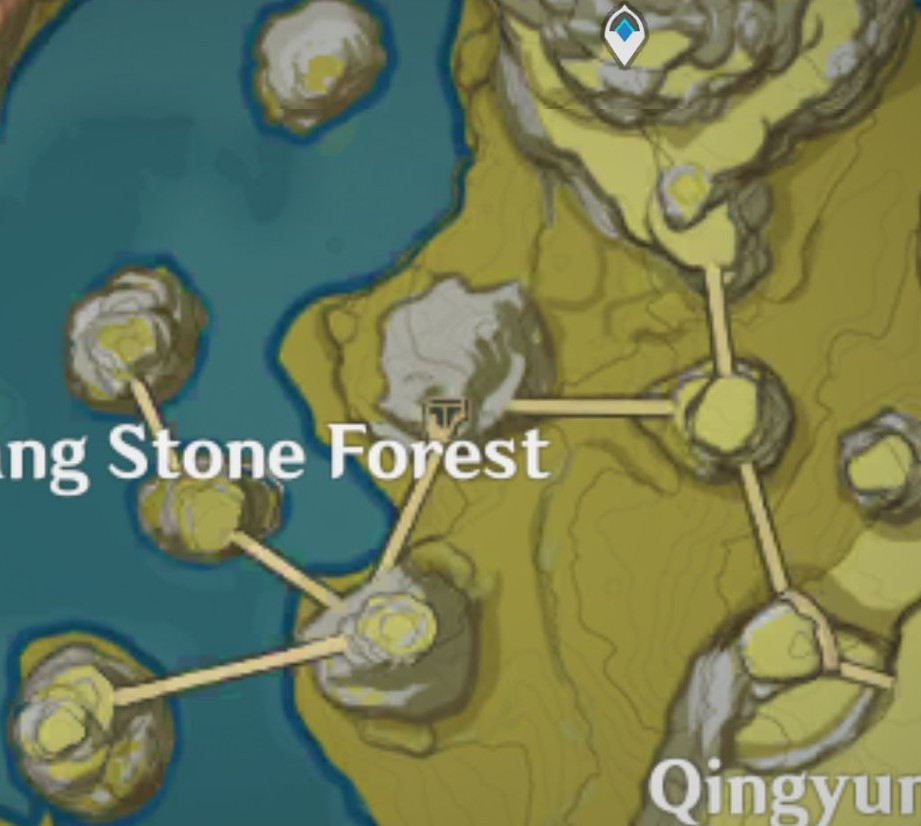
\includegraphics[scale=0.8]{path.jpg} \\
  \small{华光林}
\end{center}

最近,旅行者接到一份委托,要求旅行者去检修这些桥梁,为了使得检修时间最短,旅行者希望找到一条路径,这条路径\textbf{从传送锚点出发},恰好经过每条桥梁一次,\textbf{可以在任意山峰结束}。

你的任务是判断旅行者想要的路径是否存在。